\chapter[GPS]{Sistema de Posicionamento Global}

\begin{enumerate}
  \item \textbf{História}

  O GPS foi desenvolvido pelo Departamento de Defesa dos Estados Unidos da América, originalmente para fins militares, liberado com restrições para uso civil em 1977, e desde então vem sendo aprimorado, principalmente ao que diz respeito aos aparelhos eletrônicos e programas computacionais. \cite{usp2}

  \begin{figure}[h]
    \centering
    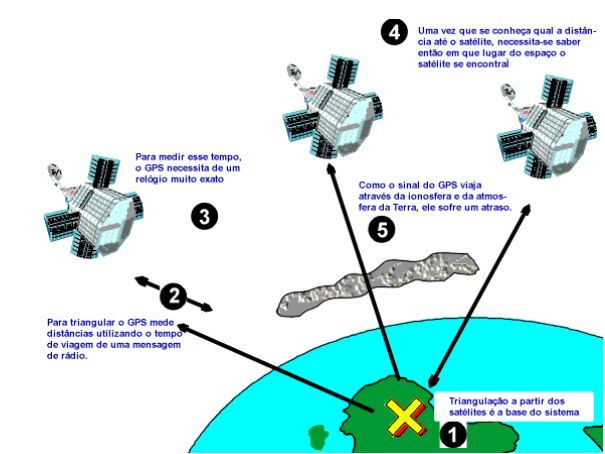
\includegraphics[width=400px, scale=0.5]{figuras/gps1}
    \label{table:gps}
  \end{figure}

  \item \textbf{As principais características do GPS são:}

  \begin{itemize}
    \item Disponibilidade contínua 24h por dia
    \item Cobertura global
    \item Latitude, Longitude, Altitude, Data-hora
    \item Precisão  $\leq$ 100 metros em 95\% do tempo
    \item Precisão diferencial sub-centimétrica
  \end{itemize}

  \item \textbf{Emissão de Sinais}

  Os sinais emitidos pelos satélites são transmitidos através de ondas (portadoras) sendo:
  \begin{itemize}
    \item L1: com freqüência 1575.42 MHz e 19 cm de comprimento de onda.
    \item L2: com freqüência de 1227.60 MHz e 24 cm de comprimento de onda.
  \end{itemize}

    Mais detalhes sobre as ondas em \cite{usp2}.

  \item \textbf{Fatores que afetam a precisão do GPS}

    \begin{itemize}
      \item  DoP

        Dilution of Precision é um termo que especifica a localização dos satélites uns em relação aos outros sob a perspectiva do receptor. Se um receptor Gps estiver localizado sob 4 satélites e todos estiverem na mesma região do céu, sua geometrica é pobre \cite{infoagro}.
        Com os mesmo 4 satélites, entretanto, com disposições diferentes no céu provém maior angulo de cobertura e aumentam drásticamente a precisão do GPS. Para maior precisão dos aparelhos GPS o valor de DoP deve ser o mais baixo possivel.

        \begin{figure}[h]
          \centering
          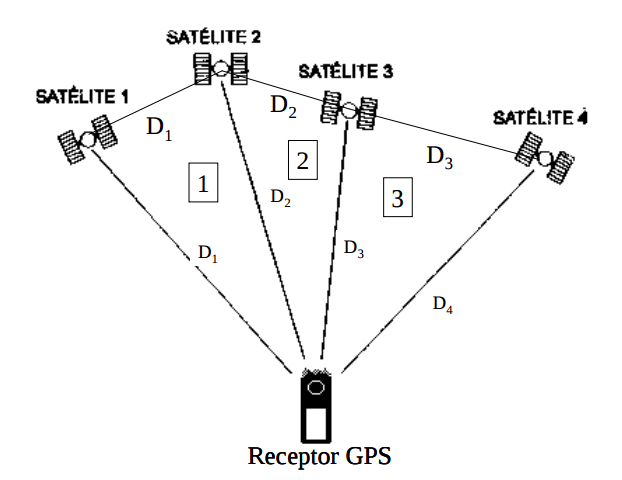
\includegraphics[width=400px, scale=0.5]{figuras/gps2}
          \label{table:gps}
        \end{figure}

      \item Multicaminhamento

      	Os sinais transmitidos pelos satélites podem sofrem diversas interferências ao longo dos seus trajetos ou antes de encontrar o receptor, gerando assim maior tempo de resposta no envio da informação e causando erros nos calculos de distância e coordenadas.
      	No caso do uso do CIAC, o parabrisas deve estar desobstruido para melhor precisão do aparelho.

      \item Local

        Devem ser evitados locais que possuam transmissão de microondas e radares, 	antenas de rádio, linhas de alta voltagem e vegetação densa. Esses fatores representam fontes de erros para o sinal GPS.

    \end{itemize}

  \item \textbf{Tipos de Aparelhos}
    \begin{itemize}
      \item Aparelhos de baixa precisão:
      
        aparelhos de uso civil, com antena interna, que identificam apenas o código C/A. Sendo geralmente o erro até 30 m sem a possibilidade de transferir os dados para o computador.
        Exclui-se a possibilidade de escolha sobre estes aparelhos pois o dispositivo a ser criado exige captação,armazenamento e transferência de dados.

      \item Aparelhos de média precisão:
      
        aparelhos de uso civil, com antena interna não amplificada, que identificam apenas a portadora L1 com o código C/A. Sendo possível transferir os dados armazenados e processá-los no método diferencial (DGPS), com erro após o processamento de alguns metros. Esses aparelhos também possibilitam configurar o setup.
        Aparelhos na faixa ideal de utilização pois correspondem ao requisito de transferência de dados e configuração externa. Além de estarem acessiveis para compra e adaptação a diferentes usos.

      \item Aparelhos de alta precisão:
      
        Excluído da pesquisa pois seu preço é alto e adaptabilidade para carros é minima.

      \item Aparelhos de altíssima precisão:
      
        Excluído da pesquisa pois seu uso é para fins militares.

    \end{itemize}
\end{enumerate}
